\subsection{Sopa de tortilla}\label{sopa_tortilla}

2 porciones\\
20 min \\


\underline{Ingredientes}
\begin{itemize}
\item 8 tortillas rebanadas en tiras y fritas en aceite
\item 1/2 cebolla
\item 2 dientes ajo
\item 2 tazas de consomé de pollo 
\item 150 gramos queso panela
\item 1 aguacate
\item 8 hojas epazote
\item 4 tomates
\item 2 chiles guajillo 
\item media crema 
\end{itemize}

\begin{figure}[H]
\centering
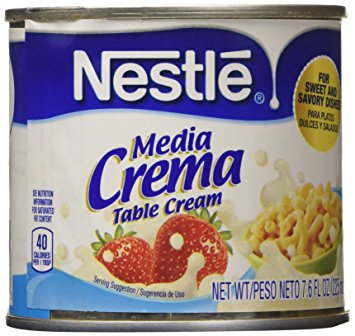
\includegraphics[scale=0.2]{recetas/sopa-de-tortilla/figures/media_crema}
\caption{Media crema. Se encuentra en Target en Baltimore Ave.}
\end{figure}

\underline{Instrucciones}
\begin{enumerate}
\item En una olla con 2 cucharadas de aceite, freír los chiles guajillo cortados en tiras pequeñas y reservar.
\item Licuar los jitomates, cebolla, ajo, 8 tiras de tortilla frita y consomé.
\item Agregar la salsa en la olla con el aceite caliente. Agegar las hojas de epazote.
\item Agregar aproximadamente 1/2 litro de agua a la olla y hervir durante 15 min.
\item Checar si hace falta agua y agregar sal al gusto. La cantidad de agua depende de la consistencia que se quiera alcanzar.
\item En un plato hondo colocar una porción de tortillas fritas y caldo.
\item Decorar con aguacate, panela, crema y tiritas de guajillo.
\end{enumerate}


\begin{figure}[H]
\centering
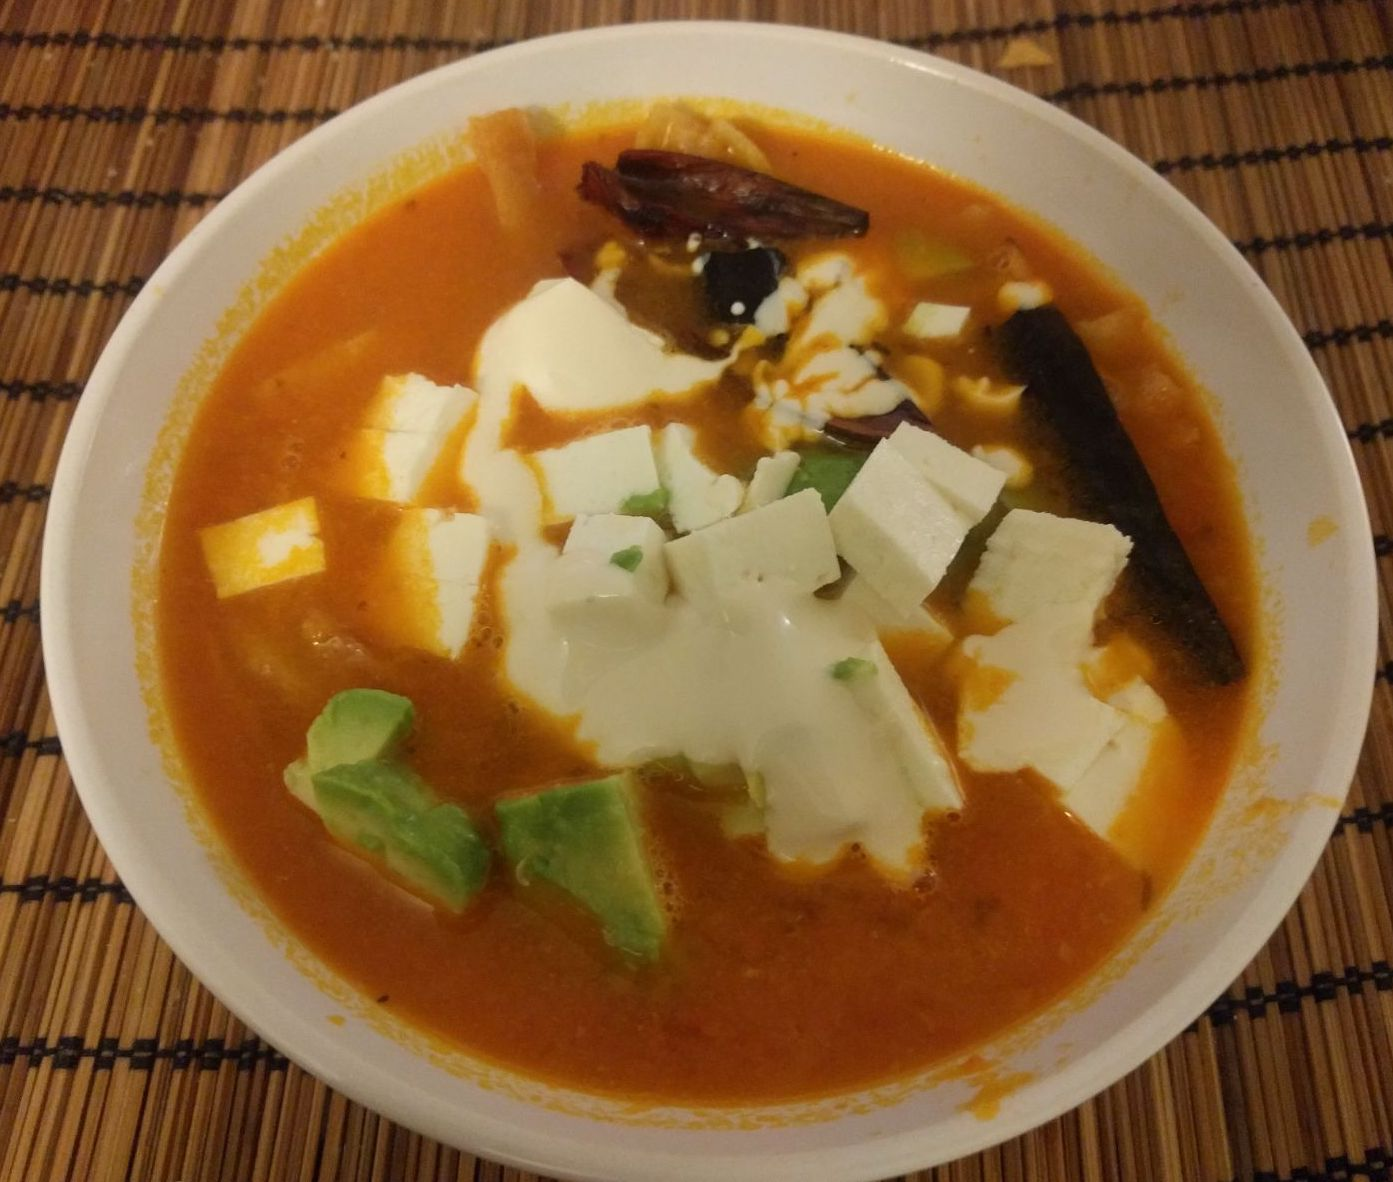
\includegraphics[scale=0.2]{recetas/sopa-de-tortilla/figures/sopa_tortilla}
\caption{Producto final}
\end{figure}

